\documentclass[12pt,a4paper]{article}
\usepackage[utf8]{inputenc}
\usepackage[portuguese]{babel}
\usepackage{graphicx}
\usepackage{subcaption}
\usepackage{geometry}
\usepackage{booktabs}
\usepackage{tabularx}
\usepackage{hyperref}
\usepackage{cite}
\usepackage{float}
\usepackage{array}
\usepackage{indentfirst}

\geometry{a4paper, margin=2cm}

\title{\textbf{Atividade 1 - Definição do\\Processo de Desenvolvimento}\\
\large MC656 - Engenharia de Software}
\author{
  Caio Lima Albuquerque - RA: 288808 \\
  Giovana Jacome Marchetti - RA: 177700 \\
  Julia de Souza Nardo - RA: 281272 \\
  Leonardo Carvalho De Luca - RA: 288820\\
  Samuel Rodrigues Ferreira - RA: 195440
}
\date{\today}

\begin{document}

\maketitle

\section{Produto e Contexto}
% BotCT
% VOTO ABERTO
% VOTO POR INDICAÇÃO
% MECANICAS ALEATORIAS BCT

% ASSEMBLEIA
% VOTO ABERTO
% QUORUM MÍNIMO
% VOTO EM UMA DECISÃO

% VOTO AUSTRÁLIA
% VOTO ANÔNIMO
% RANKEAMENTO DE CANDIDATOS
% VOTO EM PESSOAS
%Organizador — cria e configura o proces

O nosso sistema tem 3 principais objetivos: realizar votações nos contextos de um jogo de Blood on the Clocktower, uma assembleia deliberativa do Centro Acadêmico da Computação (CACo) e uma eleição no modelo da Austrália. Esses contextos foram escolhidos por terem características consideravelmente diferentes, porém mantendo a ideia de usar uma votação para tomada de decisão. Os contextos variam em tempo, simultaneidade, voto aberto ou fechado, objetivo e método de votação.

\subsection{Contextos suportados}

\subsubsection{Blood on the Clocktower}
Blood on the Clocktower~\cite{bloodontheclocktower} é um jogo de dedução social em que eliminações ocorrem por meio de votações sequenciais coordenadas por um mestre. Na fase de nomeações, um jogador acusa o outro, que tem direito a defesa. Em seguida, a votação ocorre no sentido horário: o mestre passa por cada jogador na roda e contabiliza o voto daqueles que estiverem com a mão levantada na sua vez, encerrando quando chegar no voto de quem foi acusado.

Para ir à forca, o acusado precisa de votos de pelo menos 50\% dos jogadores vivos. Se a forca já estiver ocupada, o novo acusado precisa de mais votos que o atual para substituí-lo. Caso haja um empate com os votos de quem já está na forca, ambos se salvam e a forca fica vazia. Ao final do dia, quem permanecer na forca é executado.

Nossa ideia de implementação é retirar o mestre da fase de votação, automatizando-a e inserindo um tempo limite fixo, assim os jogadores podem alternar seu status na votação (mão levantada ou abaixada) na interface até que o tempo acabe, quando a opção escolhida no momento será a contabilizada. O diferencial do sistema será exibir em tempo real o histórico dos votos já registrados e a intenção de voto (status atual da mão) dos jogadores que ainda aguardam a sua vez na sequência.

\subsubsection{Assembleia do CACo}

As votações nas assembleias do CACo~\cite{caco2026} (Centro Acadêmico da Computação da UNICAMP) são abertas e tradicionalmente realizadas pela contagem de mãos levantadas. Durante uma deliberação, cada opção de voto é chamada individualmente para que os estudantes manifestem sua escolha. Cada participante tem direito a apenas um voto por decisão, e toda pauta deve incluir obrigatoriamente a opção de abstenção. 

Para que a tomada de decisão seja validada, exige-se um quórum mínimo de modo que a assembleia deve registrar a participação de pelo menos 10\% do total de alunos matriculados nos cursos de Engenharia e Ciência da Computação.

Na implementação, o sistema buscará replicar a transparência e a dinâmica do processo presencial. Para isso, a interface exibirá aos participantes a contagem em tempo real dos votos (simulando a percepção das mãos levantadas). Além do aspecto visual, o sistema garantirá as regras de negócio nos bastidores, bloqueando a seleção de múltiplas opções por um mesmo eleitor e calculando automaticamente se o quórum de validação foi atingido.

\subsubsection{Eleição Austrália}
O sistema de eleições da Austrália é conhecido por ser diferente do que estamos acostumados no Brasil e na maioria das repúblicas. Em vez de escolher um candidato de preferência, o eleitor deve ordenar as opções disponíveis baseado na sua prioridade.

A apuração ocorre em rodadas dinâmicas:

\begin{enumerate}

    \item Contam-se as escolhas de primeira preferência de todos os eleitores. 
    
    \item O candidato com o menor número de votos é eliminado da eleição. 
    
    \item Os votos dos eleitores que escolheram o candidato eliminado são então transferidos para a próxima preferência válida listada em cada ranking. 
\end{enumerate}
Esse processo de eliminação e redistribuição de votos se repete sucessivamente até que reste apenas um candidato, que é declarado o vencedor.

Para essa implementação, a interface precisará fornecer um mecanismo interativo e intuitivo (como arrastar e soltar ou caixas de numeração) para que o usuário consiga ordenar sua lista facilmente. O principal desafio será implementar o algoritmo iterativo de apuração, pois o sistema precisará varrer os votos computados, calcular as contagens parciais, eliminar o último colocado, reatribuir os votos válidos às próximas opções e repetir o laço de cálculo até que a condição de vitória matemática seja alcançada.

\subsection{Pressupostos e simplificações}

\subsubsection{Blood on the Clocktower}
Nessa aplicação, supomos que apenas os jogadores vivos votam e que não existem habilidades em jogo que modificam algo na votação. Além disso, os jogadores eliminados não podem nomear nem serem nomeados para a forca.

\subsubsection{Assembleia do CACo}
Podemos assumir que, na assembleia do CACo, todos os estudantes presentes são votantes e devem votar em exatamente uma opção para cada tomada de decisão.

\subsubsection{Eleição Austrália}
Para simplificar as eleições será necessário que todos os eleitores preencham completamente o ranking, sem a opção de abstenção/branco/nulo ou omitir candidatos.

\subsection{Representações visuais}

\subsubsection{Fluxo de Telas}
% --- TELA DE LOGIN (Separada) ---
\begin{figure}[H]
    \centering
    \begin{subfigure}[b]{0.49\textwidth}
        \centering
        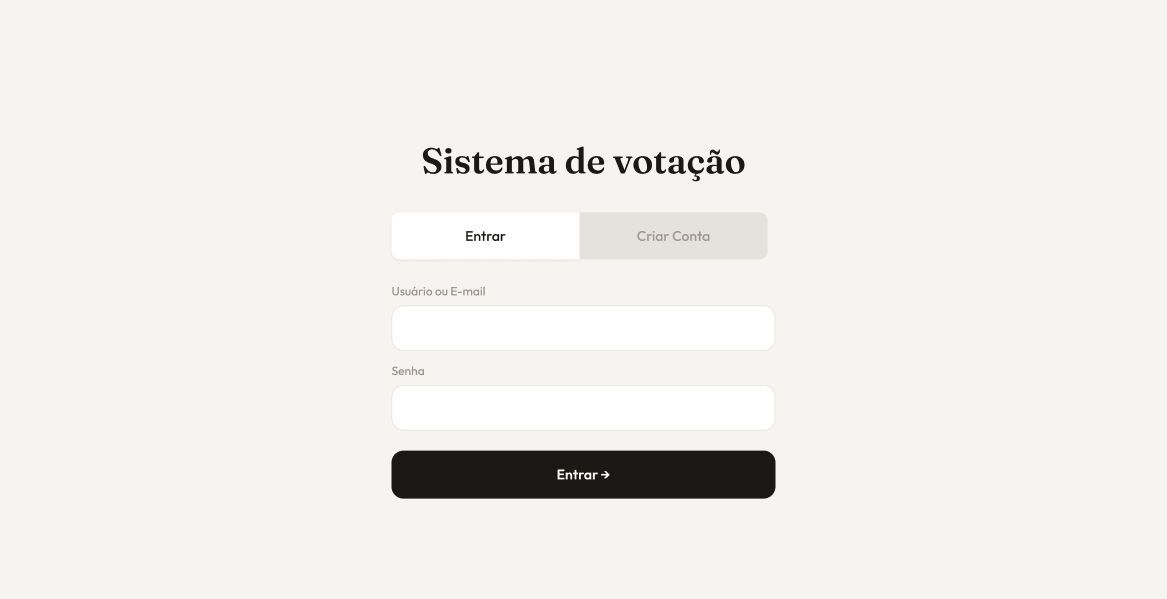
\includegraphics[width=\textwidth]{imagens/Login Page.png} 
        \caption{Tela autenticação.}
    \end{subfigure}
    \hfill
    \begin{subfigure}[b]{0.49\textwidth}
        \centering
        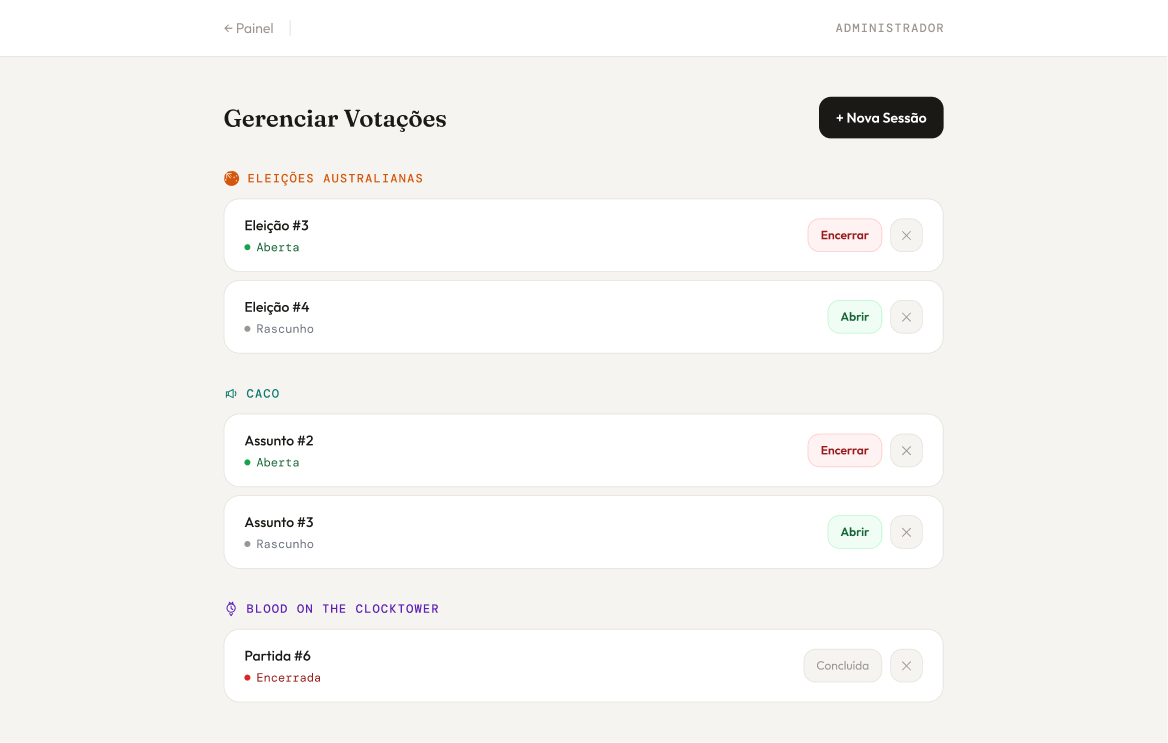
\includegraphics[width=\textwidth]{imagens/Admin Page.png} 
        \caption{Tela do administrador.}
    \end{subfigure}
    \caption{Fluxo de telas inicial e do administrador}
    \label{fig:tela_1}
\end{figure}

\vspace{1cm}

\begin{figure}[H]
    \centering
    % --- PRIMEIRA LINHA ---
    \begin{subfigure}[b]{0.45\textwidth}
        \centering
        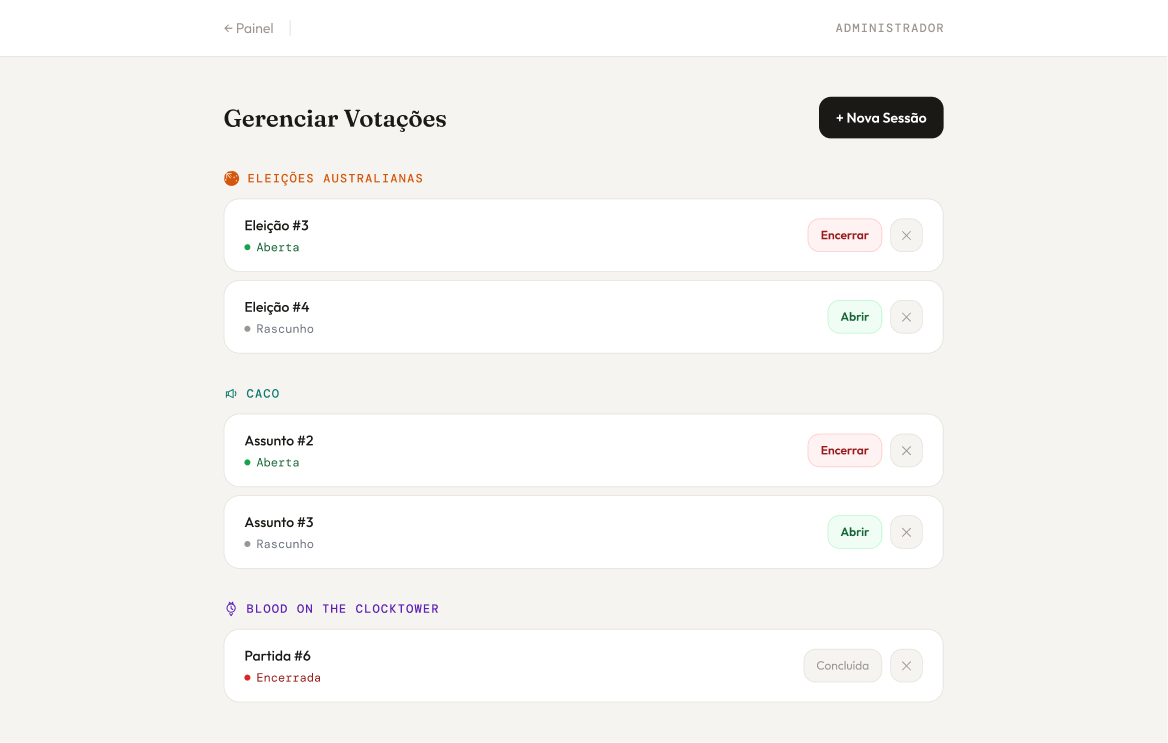
\includegraphics[width=\textwidth]{imagens/Australian Main Page.png}
        %\caption{Página Principal}
    \end{subfigure}
    \hfill
    \begin{subfigure}[b]{0.45\textwidth}
        \centering
        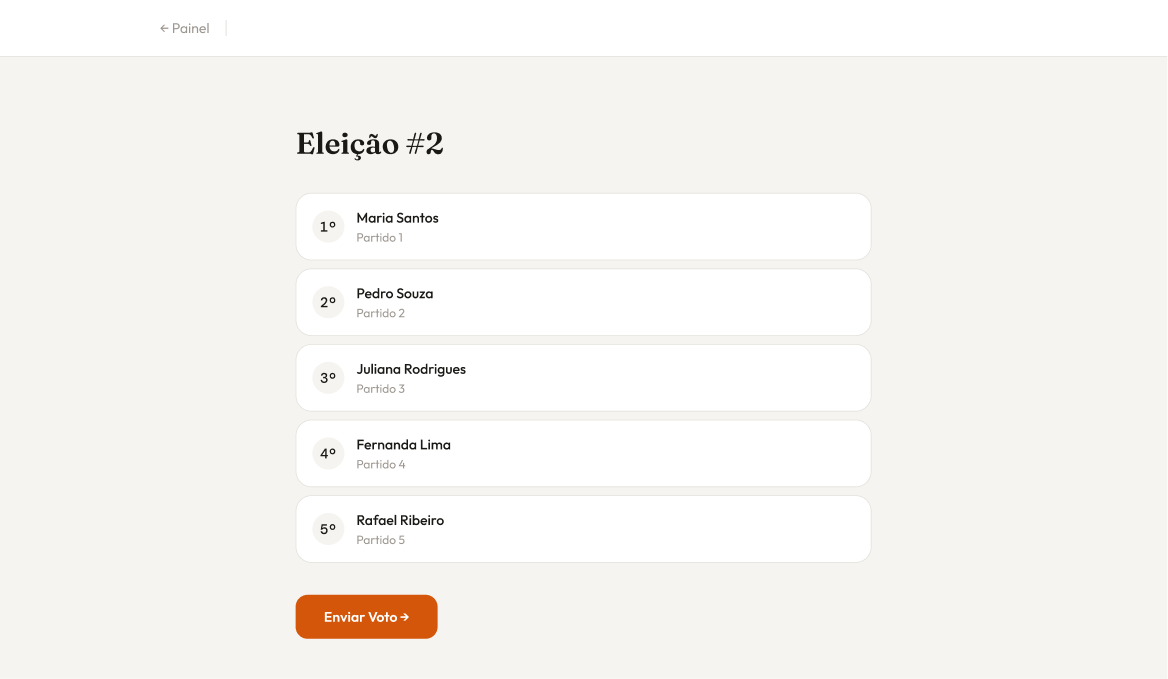
\includegraphics[width=\textwidth]{imagens/Australian Vote Page.png}
        %\caption{Votação (Rankeada)}
    \end{subfigure}
    
    \vspace{0.5cm} 
    
    % --- SEGUNDA LINHA ---
    \begin{subfigure}[b]{0.45\textwidth}
        \centering
        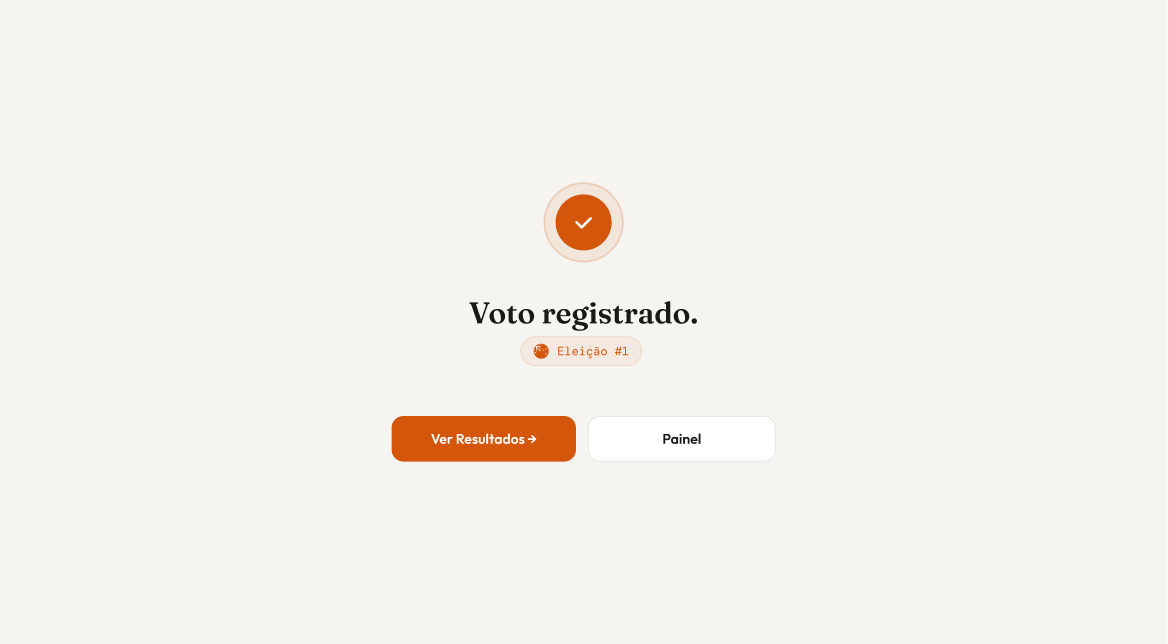
\includegraphics[width=\textwidth]{imagens/Australian Registered Page.png}
        %\caption{Confirmação}
    \end{subfigure}
    \hfill
    \begin{subfigure}[b]{0.45\textwidth}
        \centering
        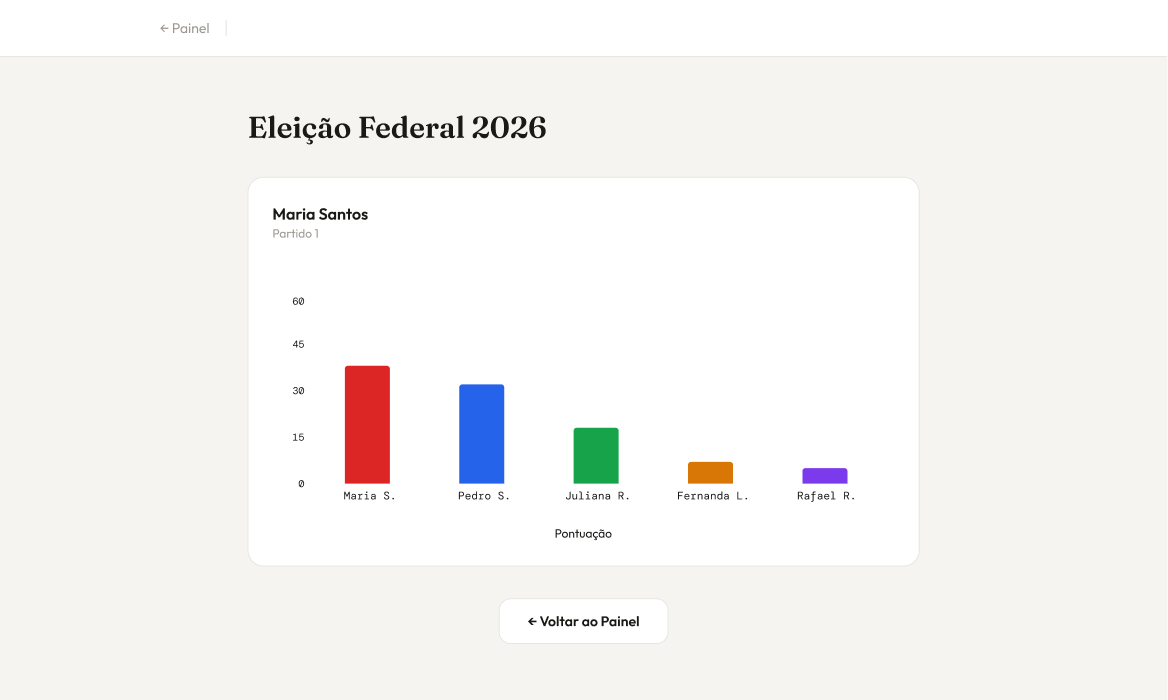
\includegraphics[width=\textwidth]{imagens/Australian Results Page.png}
        %\caption{Resultados}
    \end{subfigure}
    
    \caption{Fluxo de telas para o contexto das Eleições da Austrália.}
    \label{fig:fluxo_australia}
\end{figure}

% --- FLUXO 2: ASSEMBLEIA DO CACO ---
\begin{figure}[H]
    \centering
    % --- PRIMEIRA LINHA ---
    \begin{subfigure}[b]{0.45\textwidth}
        \centering
        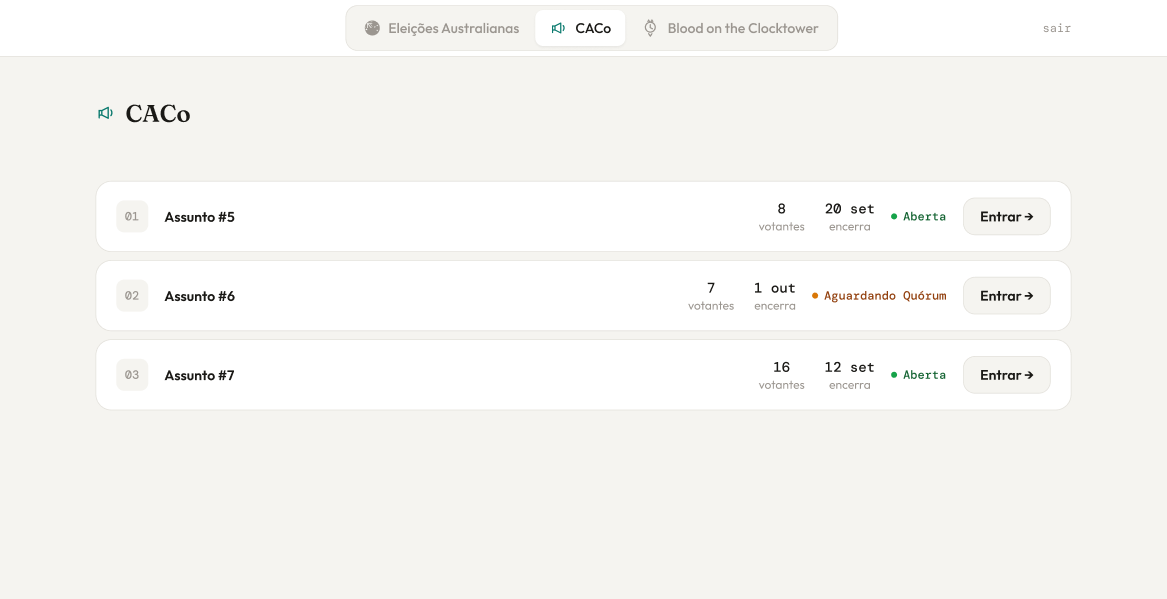
\includegraphics[width=\textwidth]{imagens/CACo Main Page.png}
        %\caption{Página Principal}
    \end{subfigure}
    \hfill
    \begin{subfigure}[b]{0.45\textwidth}
        \centering
        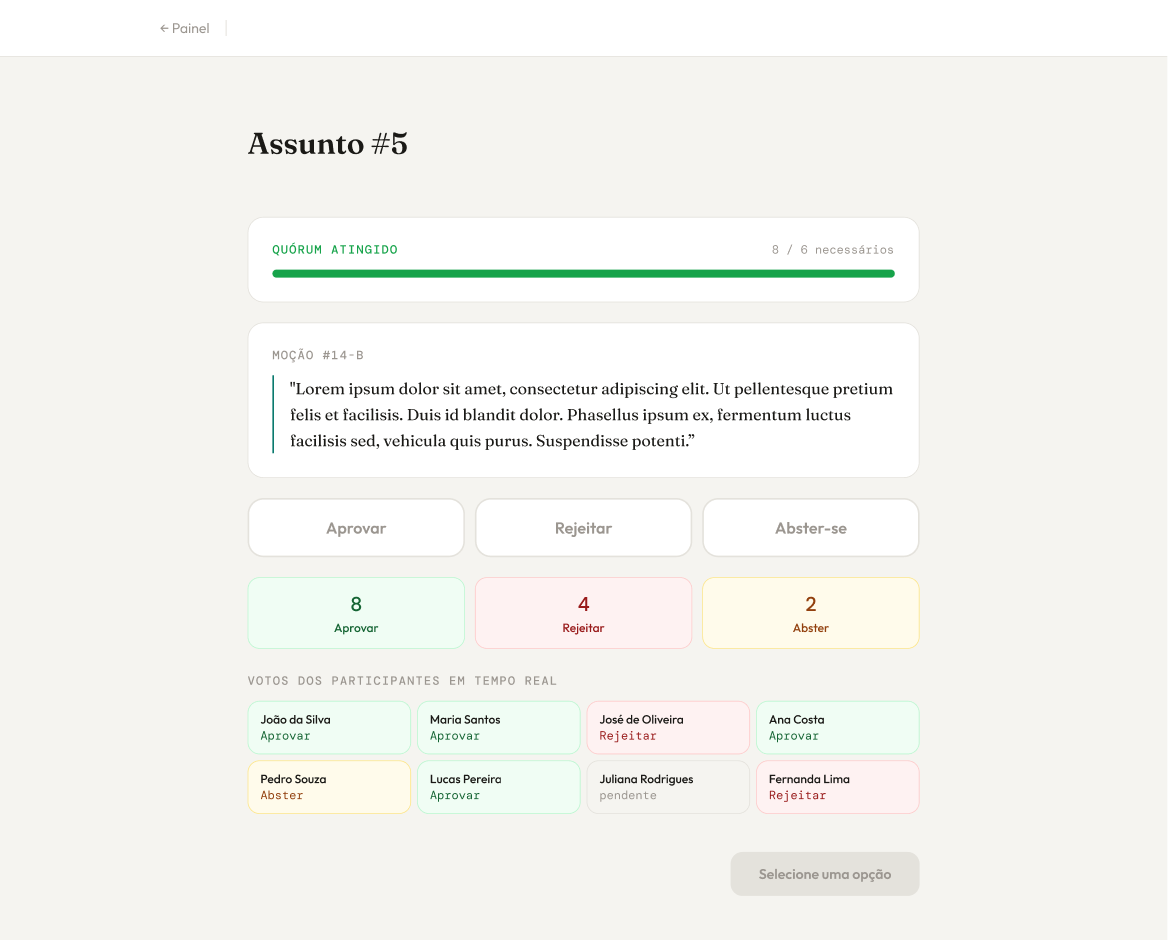
\includegraphics[width=\textwidth]{imagens/CACo Vote Page.png}
        %\caption{Votação (Aberta)}
    \end{subfigure}
    
    \vspace{0.5cm} 
    
    % --- SEGUNDA LINHA ---
    \begin{subfigure}[b]{0.45\textwidth}
        \centering
        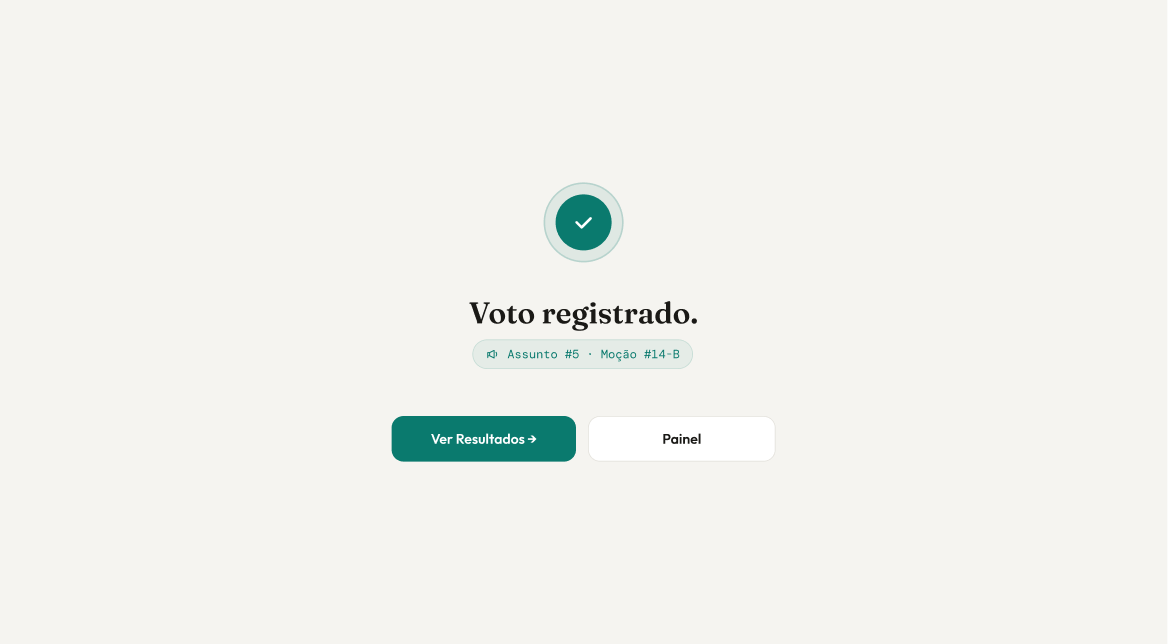
\includegraphics[width=\textwidth]{imagens/CACo Registered Page.png}
        %\caption{Confirmação}
    \end{subfigure}
    \hfill
    \begin{subfigure}[b]{0.45\textwidth}
        \centering
        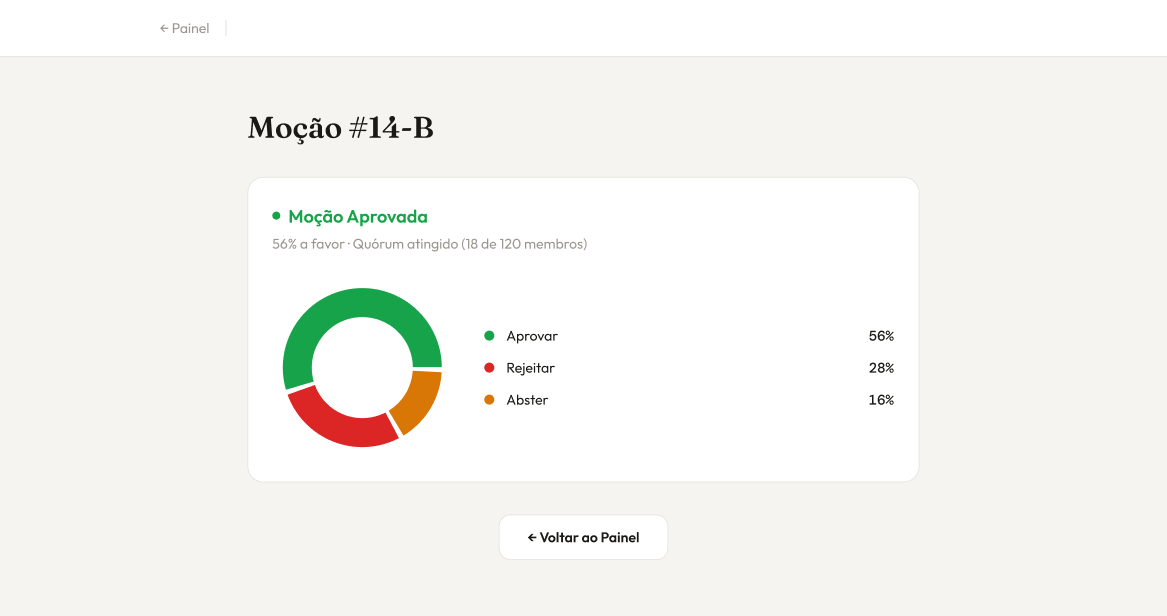
\includegraphics[width=\textwidth]{imagens/CACo Results Page.png}
        %\caption{Validação de Quórum}
    \end{subfigure}
    
    \caption{Fluxo de telas para as Assembleias do CACo.}
    \label{fig:fluxo_caco}
\end{figure}

% --- FLUXO 3: BLOOD ON THE CLOCKTOWER ---
\begin{figure}[H]
    \centering
    % --- PRIMEIRA LINHA ---
    \begin{subfigure}[b]{0.45\textwidth}
        \centering
        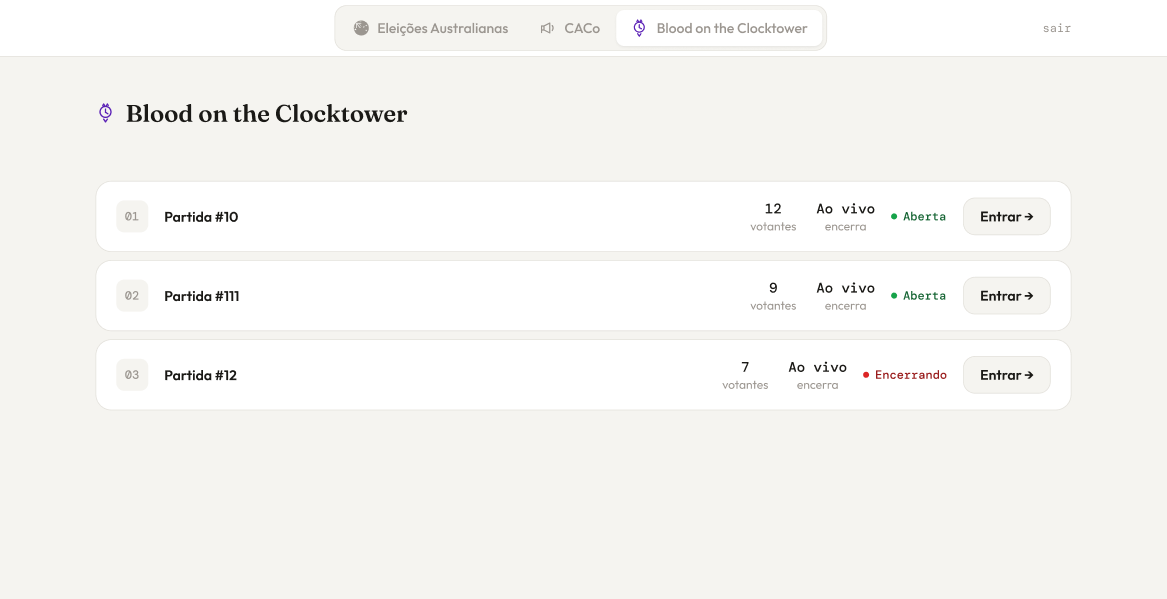
\includegraphics[width=\textwidth]{imagens/BotCT Main Page.png}
        %\caption{Página Principal}
    \end{subfigure}
    \hfill
    \begin{subfigure}[b]{0.45\textwidth}
        \centering
        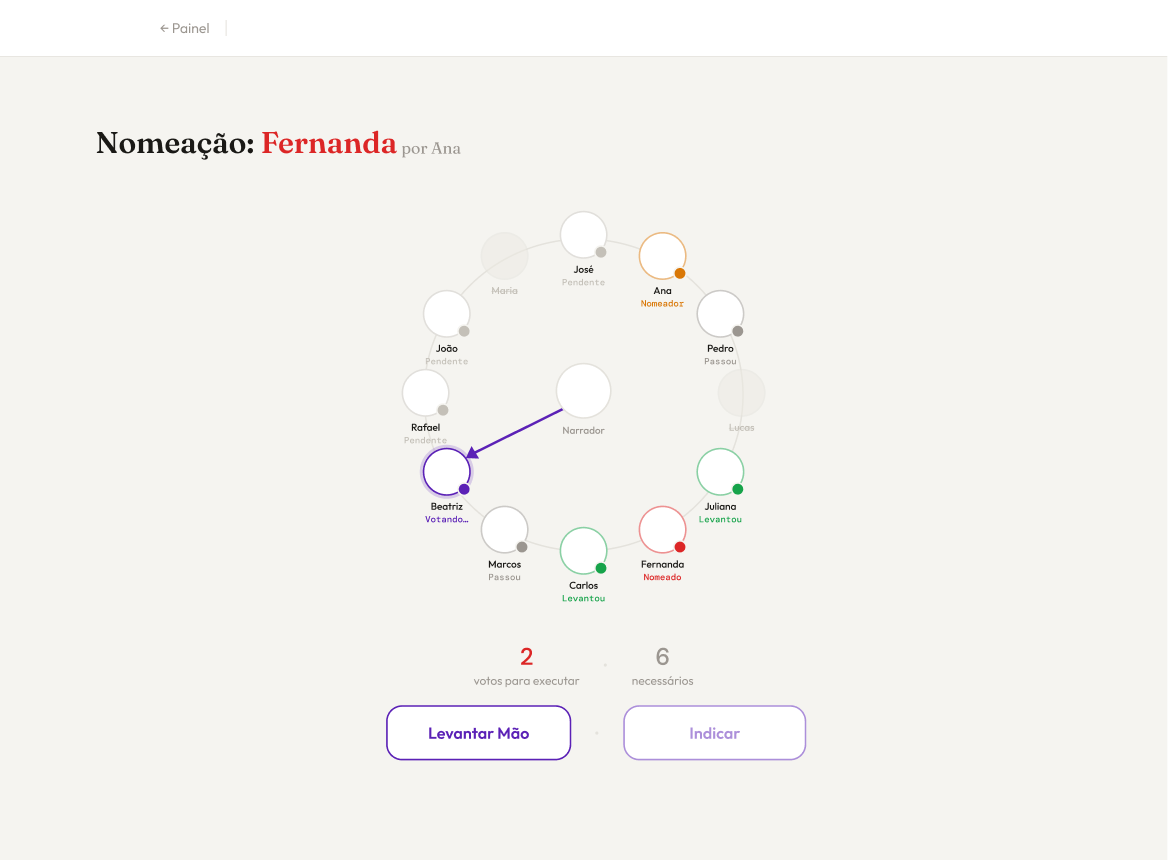
\includegraphics[width=\textwidth]{imagens/BotCT Vote Page.png}
        %\caption{Votação (Forca)}
    \end{subfigure}
    
    \vspace{0.5cm} 
    
    % --- SEGUNDA LINHA ---
    \begin{subfigure}[b]{0.45\textwidth}
        \centering
        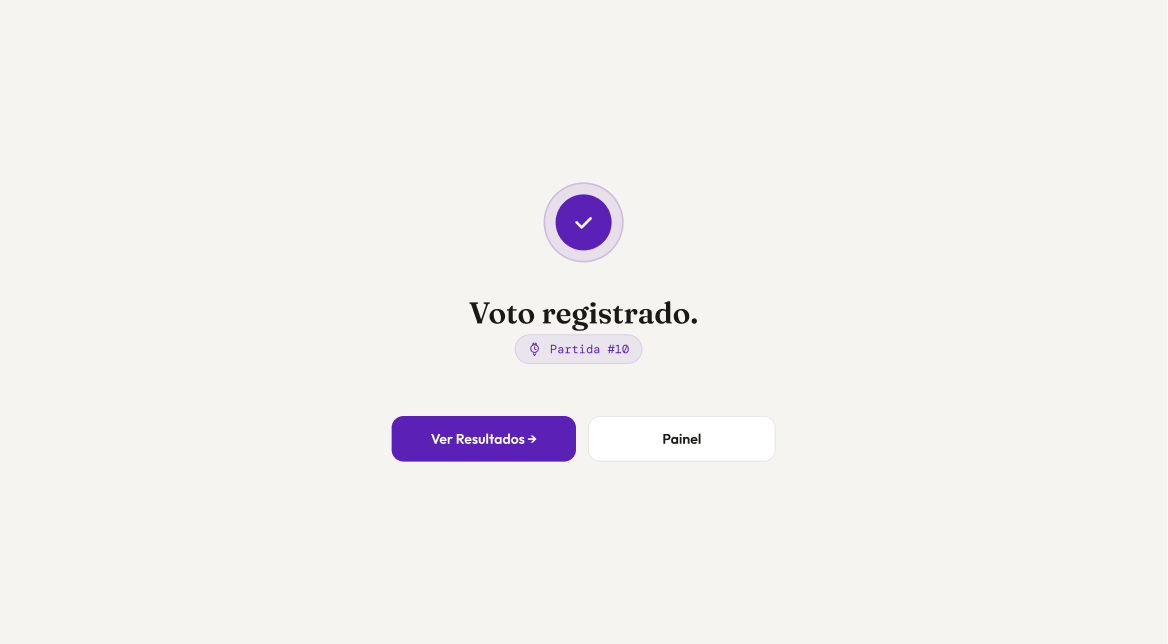
\includegraphics[width=\textwidth]{imagens/BotCT Registered Page.png}
        %\caption{Voto Computado}
    \end{subfigure}
    \hfill
    \begin{subfigure}[b]{0.45\textwidth}
        \centering
        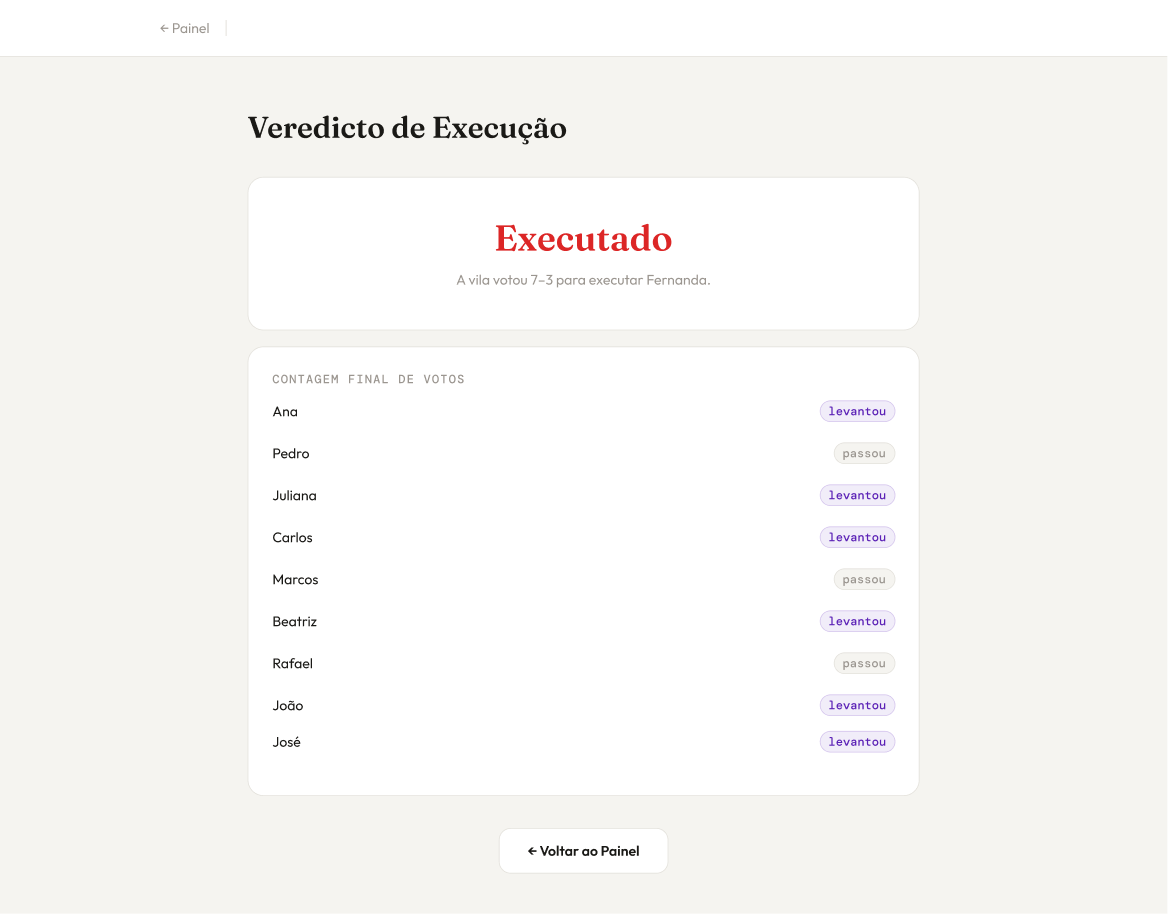
\includegraphics[width=\textwidth]{imagens/BotCT Results Page.png}
        %\caption{Status da Execução}
    \end{subfigure}
    
    \caption{Fluxo de telas para a dinâmica de Blood on the Clocktower.}
    \label{fig:fluxo_botc}
\end{figure}

\subsubsection{Diagrama de Casos}
\begin{figure}[ht]
    \centering
    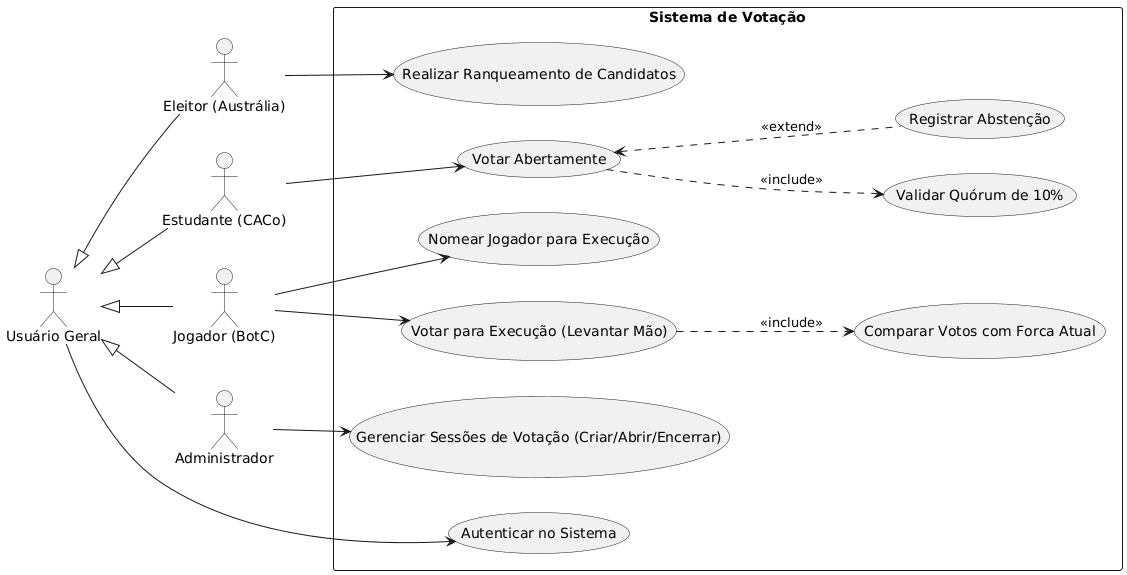
\includegraphics[width=\textwidth]{imagens/diagrama_casos.png}
    \caption{Diagrama de Casos do produto.}
\end{figure}

\subsubsection{Modelo de Domínio}
\begin{figure}[H]
    \centering
    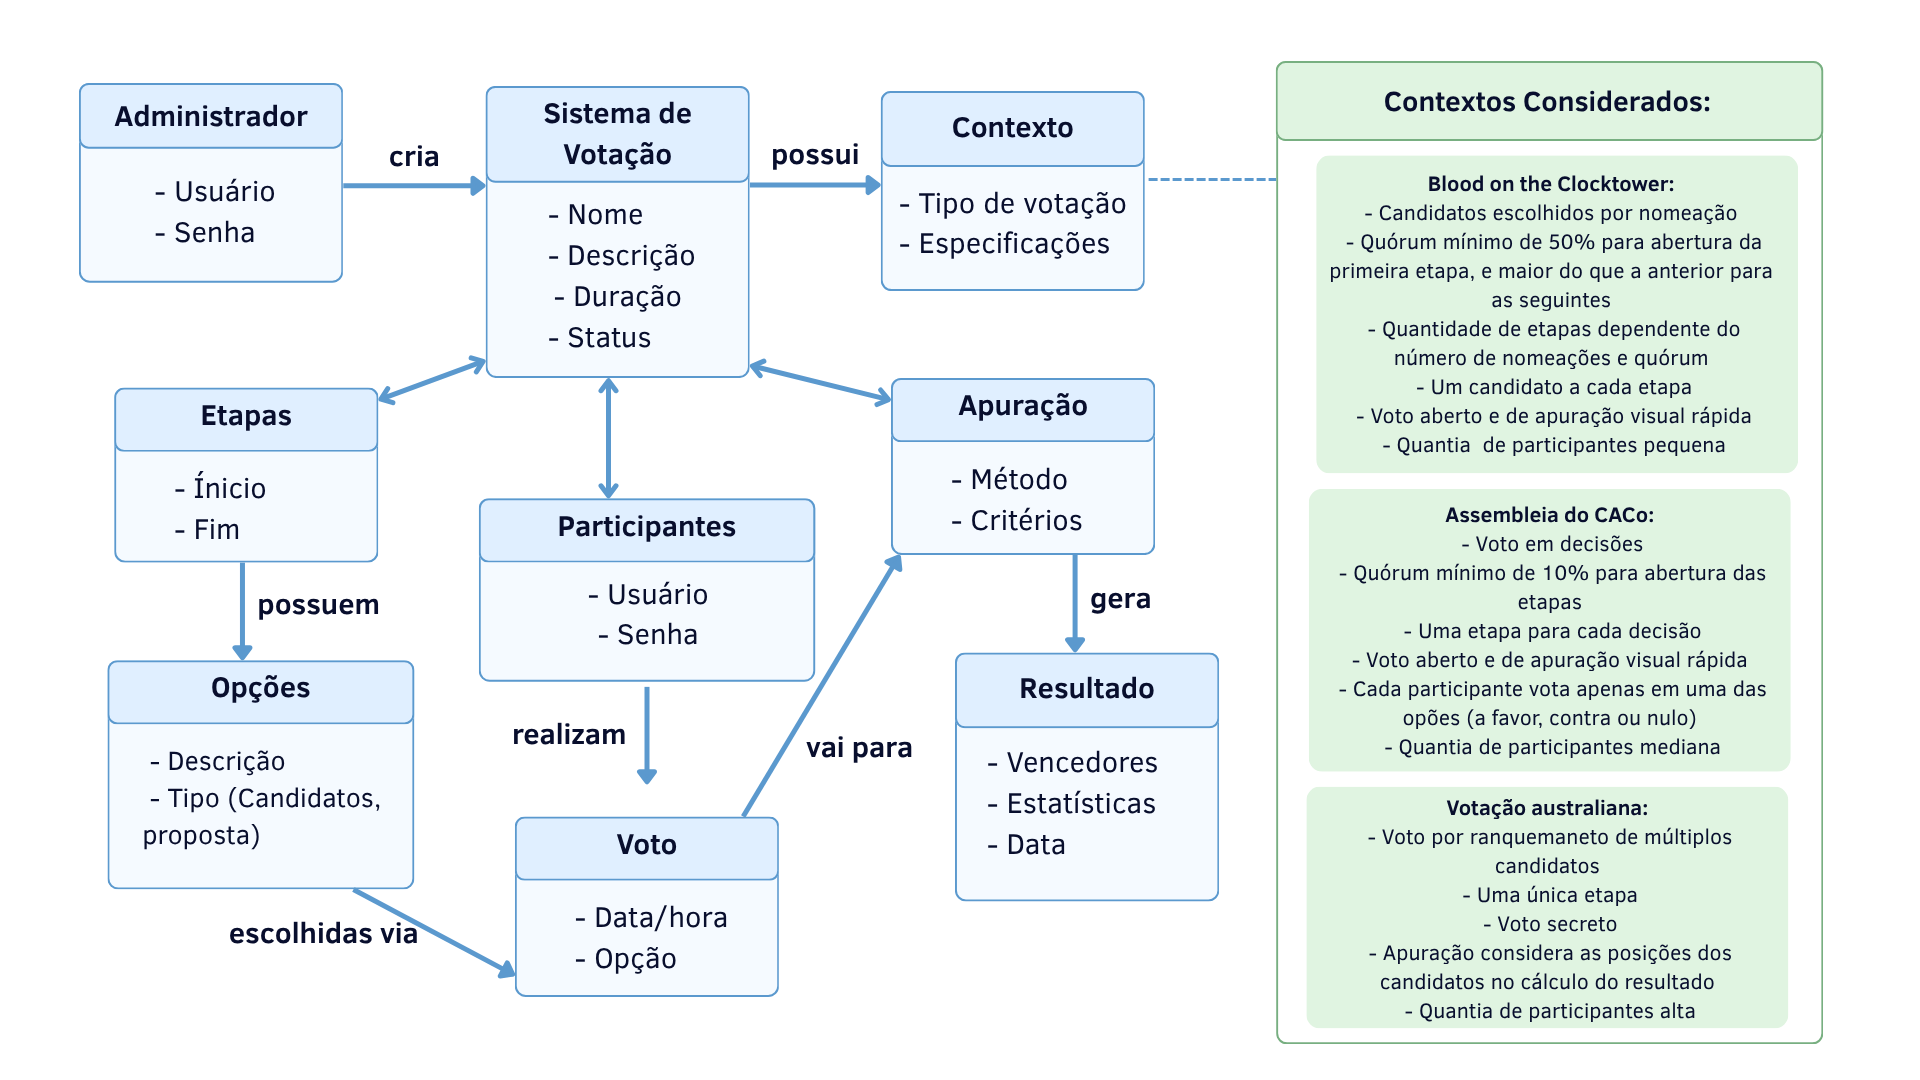
\includegraphics[width=\textwidth]{imagens/diagramadominio.png}
    \caption{Modelo de domínio do sistema de decisão coletiva.}
\end{figure}

\section{Processo de Desenvolvimento}
Para o desenvolvimento do nosso sistema, adotamos um processo iterativo e incremental em ciclos curtos de duas semanas (\textit{sprints}) baseado em Scrum~\cite{sommerville2015}. Essa escolha se justifica pelas características do nosso projeto de lidar com regras de negócio altamente distintas. É provável que, por exemplo, ao implementar o sistema de limiar móvel do \textit{Blood on the Clocktower}, a equipe descubra que a estrutura de banco de dados pensada inicialmente não atenda bem ao ranqueamento da Eleição Austrália. O Scrum nos permite identificar esses problemas arquiteturais cedo, desta forma, uma nova necessidade de refatoração do conjunto de regras poderá entrar no fluxo da equipe já na próxima \textit{sprint}, sem que o desenvolvimento de uma interface (como a simulação visual de mãos levantadas do CACo, por exemplo) fique travado esperando uma especificação perfeita e finalizada de todos os três módulos, visando uma entrega contínua de novas funcionalidades e refinamentos e garantindo previsibilidade e pontos de inspeção contínuos~\cite{fowler2001}.

Além disso, a abertura para \textit{early feedbacks} é compatível com o formato da disciplina, possibilitando uma interação constante e fácil visualização dos avanços do projetos. Da mesma forma, a valorização de entregas frequentes e simplificações de design é coerente com o prazo determinado para conclusão, viabilizando a entrega de um software funcional em poucos meses.

O trabalho se inicia no gerenciamento do \textit{Product Backlog} via \href{https://www.atlassian.com/br/software/jira}{Jira}, onde os requisitos dos três contextos são traduzidos em \textit{User Stories}. Uma funcionalidade só entra em desenvolvimento se seus Critérios de Aceite estiverem claros (ex: ``O sistema deve bloquear a apuração da Assembleia se o quórum de 10\% dos alunos de graduação não for atingido'').

O ciclo de vida de uma tarefa obedece ao seguinte fluxo: ela é alterada para \textit{In Progress} por um desenvolvedor e ramificada no GitHub a partir da branch \textit{develop}, que será mencionada a seguir. Ao finalizar a implementação local, o desenvolvedor abre um \textit{Pull Request} (PR), o qual só pode ser mesclado após a revisão de código (\textit{Code Review}) por, no mínimo, um segundo integrante da equipe que não tenha participado do desenvolvimento do código, verificando a lógica e a clareza dele~\cite{pressman2016}.

\subsection{Integração de DevOps}
A equipe adota práticas de DevOps voltadas para a Integração e Entrega Contínuas (CI/CD) utilizando o GitHub e o GitHub Actions. O fluxo de versionamento segue um modelo estruturado de acordo com o Gitflow~\cite{driessen2010gitbranching} adaptado a CI/CD de modo que: 

\begin{itemize}
    \item \textbf{\textit{main}:} Representa o ambiente de produção (ou entrega final). Contém exclusivamente código testado, estável e livre de erros. É protegida contra \textit{commits} diretos.
    
    \item \textbf{\textit{develop}:} Atua como o ambiente principal de integração. É a ramificação base onde todas as novas funcionalidades se encontram antes de serem promovidas para a \textit{main} ao final de uma \textit{sprint}.
    
    \item \textbf{\textit{feature/*}:} Ramificações temporárias criadas sempre a partir da \textit{develop} para o desenvolvimento isolado de cada tarefa (ex: \textit{feature/contagem-votos}). Garantem que o trabalho em andamento de uma sub-equipe não quebre o código dos demais. 
    
    \item \textbf{\textit{hotfix/*}:} Reservadas para situações de emergência. São criadas a partir da \textit{main} para corrigir falhas críticas de forma imediata, sendo posteriormente integradas tanto na \textit{main} quanto na \textit{develop} para manter o histórico alinhado.
    
    \item \textbf{OBS: \textit{release/*} adaptada:} No modelo Gitflow tradicional, utiliza-se branches de \textit{release} para preparação de entregas. Contudo, devido à integração com DevOps e pipelines automatizados de CI/CD (GitHub Actions), o grupo optou por suprimir essa ramificação. A validação, testes e homologação ocorrem diretamente nos Pull Requests antes do merge para a \textit{develop}, tornando a transição da \textit{develop} para a \textit{main} ao final da \textit{sprint} direta, contínua e sem ambiguidades.
\end{itemize}

Para garantir a qualidade e evitar a quebra do sistema, a branch \textit{develop} possui regras de proteção. Nenhum código é inserido diretamente nela, a integração ocorre exclusivamente via \textit{Pull Requests} (PRs) como citado anteriormente. Além disso, iremos configurar um pipeline no GitHub Actions que compila automaticamente o projeto a cada novo push. O \textit{merge} só é liberado se os testes automatizados passarem e o revisor aprovar, mantendo a branch \textit{main} estritamente para entregas estáveis e prontas para uso.

\subsection{Integração de BizDev}
O BizDev é incorporado à nossa rotina para garantir que as decisões de código reflitam com exatidão as regras complexas de cada contexto eleitoral. Essa ponte entre negócio e desenvolvimento é feita diretamente no \href{https://www.atlassian.com/br/software/jira}{Jira}.

Durante o Sprint Planning, não tratamos as tarefas apenas como desafios técnicos de programação. Cada \textit{User Story} precisa conter os ``Critérios de Aceite'' traduzidos das regras de negócio reais (ex. como o quórum mínimo de uma assembleia deve bloquear a apuração). Se durante a \textit{sprint} um desenvolvedor identificar que alguma regra é tecnicamente inviável no tempo hábil da disciplina, a equipe aciona um ciclo rápido de validação entre si para simplificar a regra sem descaracterizar o escopo da eleição. Isso garante que o esforço da equipe gere valor funcional, e não apenas fidelidade excessiva a casos extremos e aplicações genéricas.

\section{Aplicação dos Conceitos de Processo de Software}

\subsection*{Tabela 1: Caracterização das atividades}
\begin{table}[H]
\centering
\begin{tabularx}{\textwidth}{|l|l|X|X|}
\hline
\textbf{Atividade} & \textbf{Classificação} & \textbf{Objetivo} & \textbf{Quando/condição} \\ \hline
Sprint Planning & Fundamental & Definir as prioridades, traduzir regras de negócio e selecionar as tarefas do ciclo. & Primeiro dia da sprint. \\ \hline
Desenvolvimento & Fundamental & Implementar as regras e fluxos de tela definidos nas User Stories e na Sprint Backlog. & Quando uma tarefa é movida para ``In Progress'' no Jira. \\ \hline
Code Review & Guarda-chuva & Assegurar a qualidade do código e o funcionamento da CI. & Sempre que um novo PR é aberto \\ \hline
Sprint Review & Fundamental & Avaliar as funcionalidades entregues, alinhar com BizDev e adaptar o planejamento. & Último dia da sprint. \\ \hline
\end{tabularx}
\end{table}

\subsection*{Tabela 2: Execução das atividades}
\begin{table}[H]
\centering
\begin{tabularx}{\textwidth}{|l|l|X|X|X|}
\hline
\textbf{Atividade} & \textbf{Participantes} & \textbf{Recursos} & \textbf{Entradas} & \textbf{Resultados} \\ \hline
Sprint Planning & Toda a equipe & Jira & Product Backlog, User Stories & Sprint Backlog \\ \hline % OIIIII SAMUEEEEEEEEEEEEEL
Desenvolvimento & Desenvolvedores & IDE, Git & Sprint Backlog, User Stories & Código-fonte \\ \hline
Code Review & Revisores (não autores) & GitHub, GitHub Actions & Código-fonte & Feedback \\ \hline
Sprint Review & Toda a equipe & Localhost & Código-fonte, Sprint Backlog, Product Backlog & Incremento de código validado, Feedback, Release \\ \hline
\end{tabularx}
\end{table}

\subsection*{Tabela 3: Artefatos do processo}

\begin{table}[H]
\centering
\begin{tabularx}{\textwidth}{|l|X|X|}
\hline
\textbf{Artefato} &
\textbf{Finalidade} &
\textbf{Atividades em que é criado, atualizado ou utilizado} \\
\hline

Product Backlog &
Registrar necessidades do produto. &
Sprint Planning; Sprint Review \\
\hline

User Stories &
Descrever as funcionalidades do sistema a partir das necessidades dos usuários. &
Sprint Planning; Desenvolvimento \\
\hline

Sprint Backlog &
Guiar o trabalho da equipe durante a Sprint, reunindo as tarefas selecionadas para desenvolvimento. &
Sprint Planning; Desenvolvimento; Sprint Review \\
\hline

Código-fonte &
Implementar as funcionalidades e regras do sistema, com uso de Commits e Pull Requests.  &
Desenvolvimento; Code Review; Sprint Review \\
\hline

Incremento de código validado &
Representar a versão funcional do sistema produzida ao longo da Sprint e disponibilizada para validação. &
Sprint Review \\
\hline

Feedback &
Registrar sugestões, problemas e necessidades identificadas durante a validação do incremento. &
Sprint Review; Code Review \\
\hline

Release &
Representar uma versão estável do sistema destinada à entrega. &
Sprint Review \\
\hline

\end{tabularx}
\end{table}


\section{Representação Visual do Processo}
\begin{figure}[ht]
    \centering
    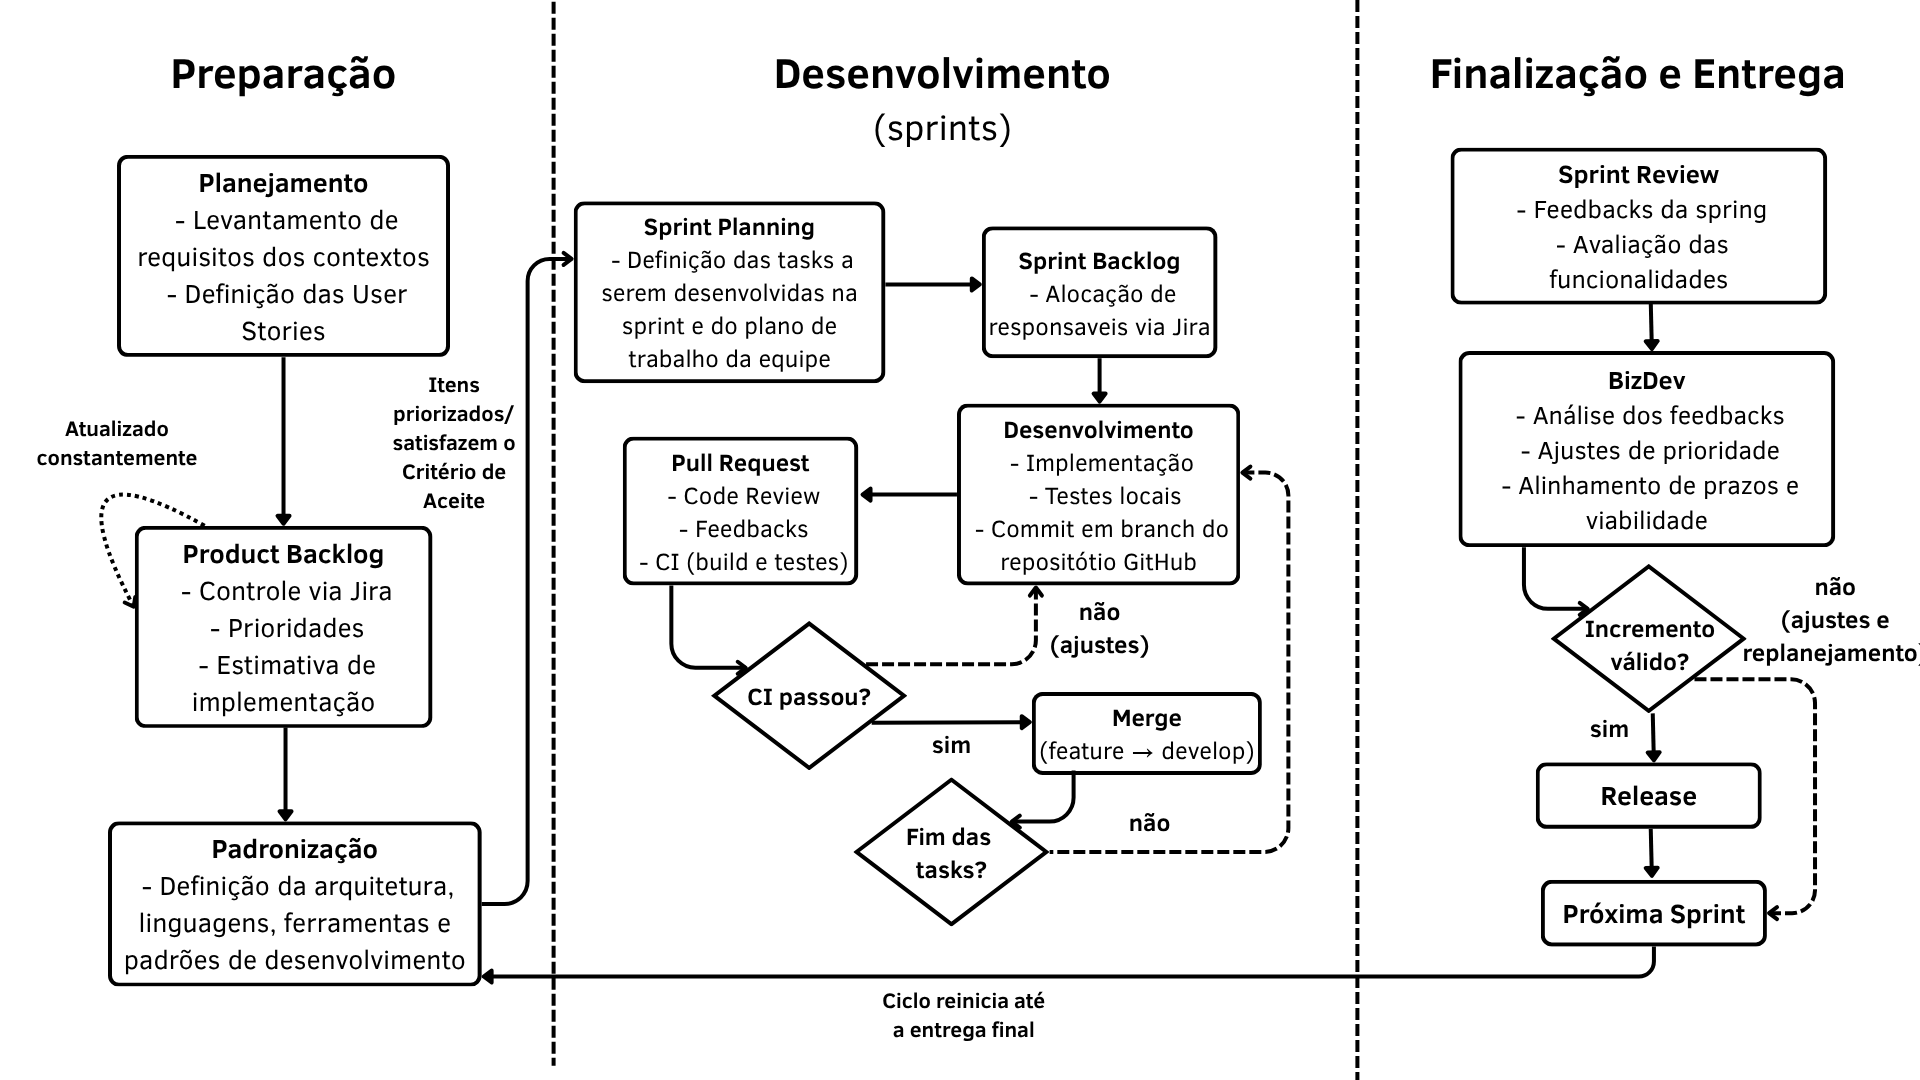
\includegraphics[width=\textwidth]{imagens/processos.png}
    \caption{Fluxo do Processo de Desenvolvimento da Equipe.}
\end{figure}

\bibliography{references}
\bibliographystyle{plain}

\end{document}